% titlepages
\begin{titlepage}
	\centering
	% left bottom right top
%	\includegraphics[trim = 20mm 100mm 20mm 20mm, clip, width = 50mm]{pic/title.jpg}\par\vspace{1cm} \nocite{wr}
	
	{\scshape\LARGE Hochschule Luzern \par}
	\vspace{0.75cm}
	{\scshape\Large EMANT Laborbericht 1\par}
	\vspace{1cm}
	{\huge\bfseries Monopol Antenne\par}
	\vspace{1.5cm}
	{\Large\itshape Markus Birrer\par}
	\vspace{0.5cm}
	
	\begin{figure}[htbp]
		\centering
		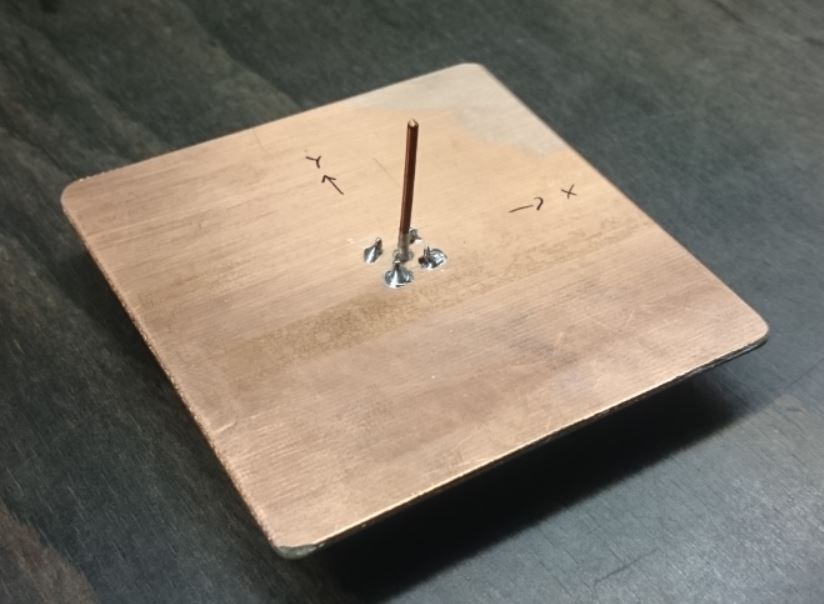
\includegraphics[width=0.6\textwidth]{pic/Monopol_Antenne.JPG}
		\label{fig:MonopolAntenne}
	\end{figure}
	
		\vspace{0.5cm}
	
	{\Large\itshape Datum Messungen: 4.Mai 2017 \par}
	
	
	\vspace*{15 mm}
	\raggedright
	{\Large Selbstständigkeitserklärung} \\
	\vspace{0.5cm}
	Hiermit erkläre ich, dass ich die vorliegende Arbeit selbstständig angefertigt und keine anderen als die angegebenen Hilfsmittel verwendet habe. Sämtliche verwendeten Textauschnitte, Zitate oder Inhalte anderer Verfasser wurden ausdrücklich als solche gekennzeichnet. \\
	\vspace{1cm}
	{\large Horw, \today      \hspace{150pt} Unterschrift:}   
	
	
  
	
	%supervised by\par
	%Dr.~Mark \textsc{Brown}

	\vfill

% Bottom of the page
%	{\large \today\par}
\end{titlepage}

\newpage


% declaration
\clearpage
\thispagestyle{empty}
\section*{Selbstständigkeitserklärung}
Hiermit erkläre ich, dass ich die vorliegende Arbeit selbstständig angefertigt
und keine anderen als die angegebenen Hilfsmittel verwendet habe. Sämtliche
verwendeten Textausschnitte, Zitate oder Inhalte anderer Verfasser wurden
ausdrücklich als solche gekennzeichnet.

\begin{table}[h!]
	\begin{tabular}{l l l}
		& & \\
		& & \\
		& & \\
		\rule{5cm}{0.25pt} & & \rule{5cm}{0.25pt} \\
		Ort, Datum & & Unterschrift
	\end{tabular}
\end{table}

\clearpage


% abstract
%\thispagestyle{empty}
\otherlanguage{english}
\begin{abstract}
%------------------------------------------------------------------------------
% Hintergrund
%------------------------------------------------------------------------------
\todo{HINTERGRUND}
% Was ist bereits bekannt zum Thema?
\todo{Was ist bereits bekannt zum Thema?}

% Was ist noch unbekannt?
\todo{Was ist noch unbekannt?}

% Was soll die Arbeit untersuchen?
\todo{Was soll die Arbeit untersuchen?}

%------------------------------------------------------------------------------
% Methode 
%------------------------------------------------------------------------------

% Wie war das Vorgehen?
\todo{Wie war das vorgehen?}

% Welche Mittel sind verwendet worden?
\todo{Welche Mittel sind verwendet worden?}

% Unter welchen Bedingungen ist untersucht worden?
\todo{Unter welchen Bedingungen ist untersucht worden?}

%------------------------------------------------------------------------------
% Ergebnisse
%------------------------------------------------------------------------------
\todo{ERGEBNISSE}

%------------------------------------------------------------------------------
% Schlussfolgerung
%------------------------------------------------------------------------------
\todo{SCHLUSSFOLGERUNGEN}

% Hauptergebnis
\todo{Hauptergebnis}

% Zusätzliche Feststellungen
\todo{Zusätzliche Feststellungen}

% Perspektiven
\todo{Perspektiven}

\end{abstract}
\otherlanguage{ngerman}

%\clearpage
% https://www.ncbi.nlm.nih.gov/pmc/articles/PMC3136027/
\thispagestyle{empty}
\begin{abstract}
%------------------------------------------------------------------------------
% Hintergrund
%------------------------------------------------------------------------------
%\todo{HINTERGRUND}
% Was ist bereits bekannt zum Thema?
\todo{Was ist bereits bekannt zum Thema?}

% Was ist noch unbekannt?
\todo{Was ist noch unbekannt?}

% Was soll die Arbeit untersuchen?
\todo{Was soll die Arbeit untersuchen?}
	
%------------------------------------------------------------------------------
% Methode 
%------------------------------------------------------------------------------

% Wie war das Vorgehen?
\todo{Wie war das vorgehen?}

%	
% Welche Mittel sind verwendet worden?
\todo{Welche Mittel sind verwendet worden?}

% Unter welchen Bedingungen ist untersucht worden?
\todo{Unter welchen Bedingungen ist untersucht worden?}

%------------------------------------------------------------------------------
% Ergebnisse
%------------------------------------------------------------------------------
\todo{ERGEBNISSE}

%------------------------------------------------------------------------------
% Schlussfolgerung
%------------------------------------------------------------------------------
\todo{SCHLUSSFOLGERUNGEN}

% Hauptergebnis
\todo{Hauptergebnis}

% Zusätzliche Feststellungen
\todo{Zusätzliche Feststellungen}

% Perspektiven
\todo{Perspektiven}

\end{abstract}


\newpage
\thispagestyle{empty} ~ % add blank page
%\shorttoc{Kapitelübersicht}{0}
%\newpage
\tableofcontents
\clearpage

% document contents
\section{Einführung}
Dieser Design Report zeigt die Vorgehensweise um einen Wireless USB-Dongle mit Sendefrequenzen von 2.4 GHz und 5 GHz zu entwickeln. Als erstes wurden Berechnungen betreffend Machbarkeit durchgeführt. Danach wurde in der Simulationsumgebung Empire ein Modell erstellt und simuliert. Über mehrere Simulationsschritte wurde das Modell verfeinert. Nach dem Herstellen des Printes folgte das Ausmessen des Printes. Dies geschah mittels Netzwerkanalyzer und dem LinearScanner Starlab. Zum Abschluss erfolgte ein Vergleich zwischen den Simulationsresultaten und den Messergebnissen.

\subsection{Erläuterungen zu den Berechnungen}
Die nachfolgenden Berechnungen waren die Grundlage für die Entwicklung des ersten Entwurfs. 
Betreffend der Freiraumdämpfung wurde ein Sendedurchmesser von 20 m gewählt. Dies resultiert in einer Freiraumdämpfung von -57 dB.\\
Über das Linkbudget ist ersichtlich, dass der Antennengewinn nicht kleiner als -6 dB sein darf.\\
Das Antennendesign benötigt nicht den gesamten zur Verfügung stehenden Platz. Mithilfe Chu's Kugel konnten die Aussenmasse der Antenne bestimmt werden. Das Harrington Gain Limit zeigt den maximal möglichen Gewinn der Antenne. Berechnet wurden 0.2 dB, in der Praxis dürfte der Wert tiefer liegen. Er sollte aber wie erwähnt nicht tiefer als -6 dB liegen.




\clearpage
\section{Experimentelles}

%\todo{Dieser Teil enthält die Liste der verwendeten Geräte, der
%	Versuchsaufbau, allfällig verwendete Daten, Grafiken und
%	Berechnungen und Simulationen für die Versuchsvorbereitung
%	(Messerwartung), Versuchsablauf in Prosa, sodass ein
%	Student / Studentin den Versuch wiederholen könnte.}

\subsection{Berechnungen}

\subsubsection{Wahl der Betriebsfrequenz}

Um eine möglichst kompakte Antenne zu erhalten, ist eine hohe
Betriebsfrequenz zu wählen, denn die geometrischen Abmessungen
der Monopolantenne sind umgekehrt proportional zur Frequenz
respektive proportional zur Wellenlänge.

\begin{equation}
	l \sim \lambda = \frac{c}{f}
\end{equation}

Um also eine Monopolantenne zu erhalten, deren Stablänge $l_s$
und Kantenlänge $l_k$ möglichst klein sind, ist eine entsprechend
hohe Frequenz $f$ zu wählen. Die Betriebsfrequenz wird gewählt mit
80\% des erlaubten Spektrums.

\begin{equation}
	f
	= 0.8 \cdot f_{max}
	= 0.8 \cdot \SI{5}{\giga\hertz}
	= \SI{4}{\giga\hertz} 
\end{equation}

\subsubsection{Monopolantenne auf quadratischer Groundplane}

Für die Dimensionierung der Antenne wird die Wellenlänge benötigt,
welche sich mit der gewählten Frequenz $f$ und der Lichtgeschwindigkeit
$c$ ermitteln lässt.

\begin{equation}
	\lambda
	= \frac{c}{f}
	\approx \frac{\SI{3d8}{\meter\per\second}}{\SI{4}{\giga\hertz}}
	= \SI{75d-3}{\meter} 
\end{equation}

Aus der Aufgabenstellung geht hervor, dass die Groundplane mit einer
Diagonale $l_d$ von $\frac{\lambda}{\sqrt{2}}$ zu erstellen ist
\cite[S.1, 2a]{lab1}. Für eine quadratische Groundplane ergibt sich
die Kantenlänge $l_k$ der Groundplane somit zu $\frac{\lambda}{2}$.

\begin{equation}
	l_d
	= \sqrt{{l_k}^2 + {l_k}^2}
	= \sqrt{2 \cdot ({l_k}^2)}
	= \sqrt{2} \cdot l_k
\end{equation}

\begin{equation}
	l_k
	= \frac{l_d}{\sqrt{2}}
	= \frac{\left(\frac{\lambda}{\sqrt{2}}\right)}{\sqrt{2}}
	= \frac{\lambda}{\sqrt{2} \cdot \sqrt{2}}
	= \frac{\lambda}{2}
	= \frac{\SI{75d-3}{\meter}}{2}
	= \SI{37.5d-3}{\meter}
\end{equation}

Die Stablänge $l_s$ der Antenne ist analog zur Groundplane mit der
Frequenz $f$ respektive der Wellenlänge $\lambda$ zu ermitteln.

\begin{equation}
	l_s
	= \frac{\lambda}{4}
	= \frac{\SI{75d-3}{\meter}}{4}
	= \SI{18.8d-3}{\meter}
\end{equation}

\begin{figure}[h!]
	\centering
	\def\svgwidth{0.5\textwidth}
	\input{../fig/gph/monopol_a.pdf_tex}
	\caption{Modellzeichnung der Monopolantenne mit quadratischer
		Groundplane.}
\end{figure}

\subsection{Simulation}

\subsubsection{Aufbau}

\begin{figure}[h!]
	\centering
	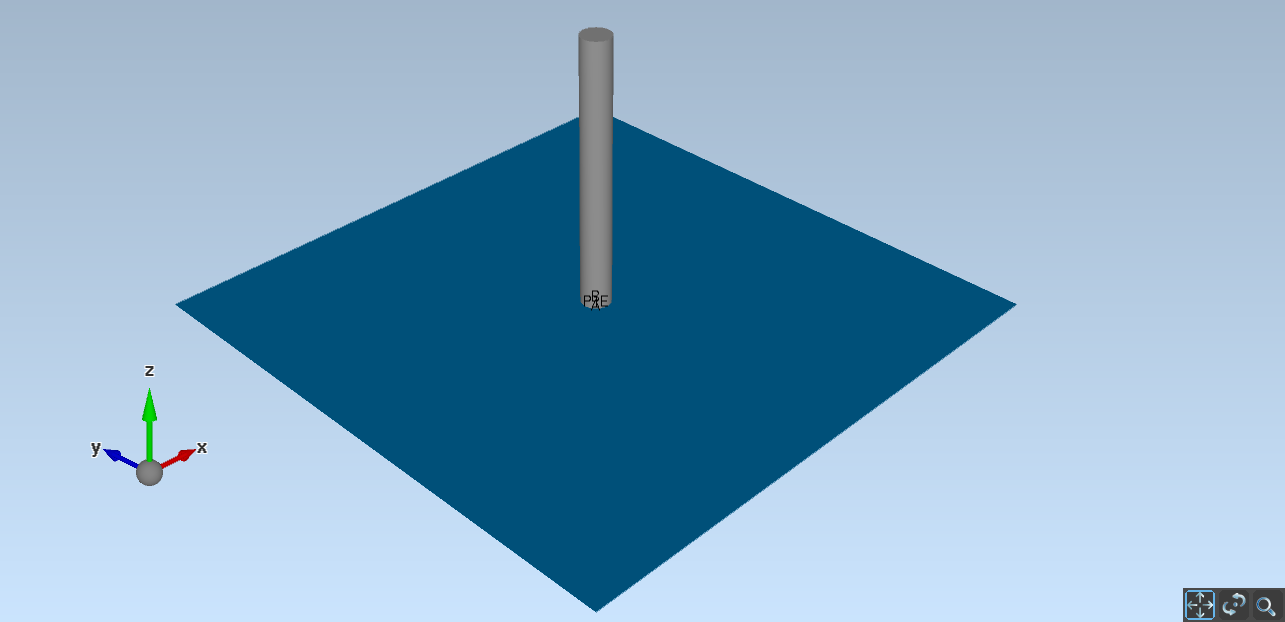
\includegraphics[width=0.75\textwidth]{../fig/plt/monopol_a_sim_3d_model.png}
	\caption{Erstelltes Simulationsmodell.}
\end{figure}

Das Simulationsmodell entspricht der zuvor vorgestellten Geometrie.
Für die Simulation wurde dem Modell noch eine Quelle hinzugefügt,
welche die Einspeisung repräsentiert. Diese ist zwischen dem
Stab und der Groundplane platziert, wodurch diese miteinander
über die Quelle verbunden werden.

\newpage
\subsubsection{Reflexionskoeffizient}

\begin{figure}[h!]
	\centering
	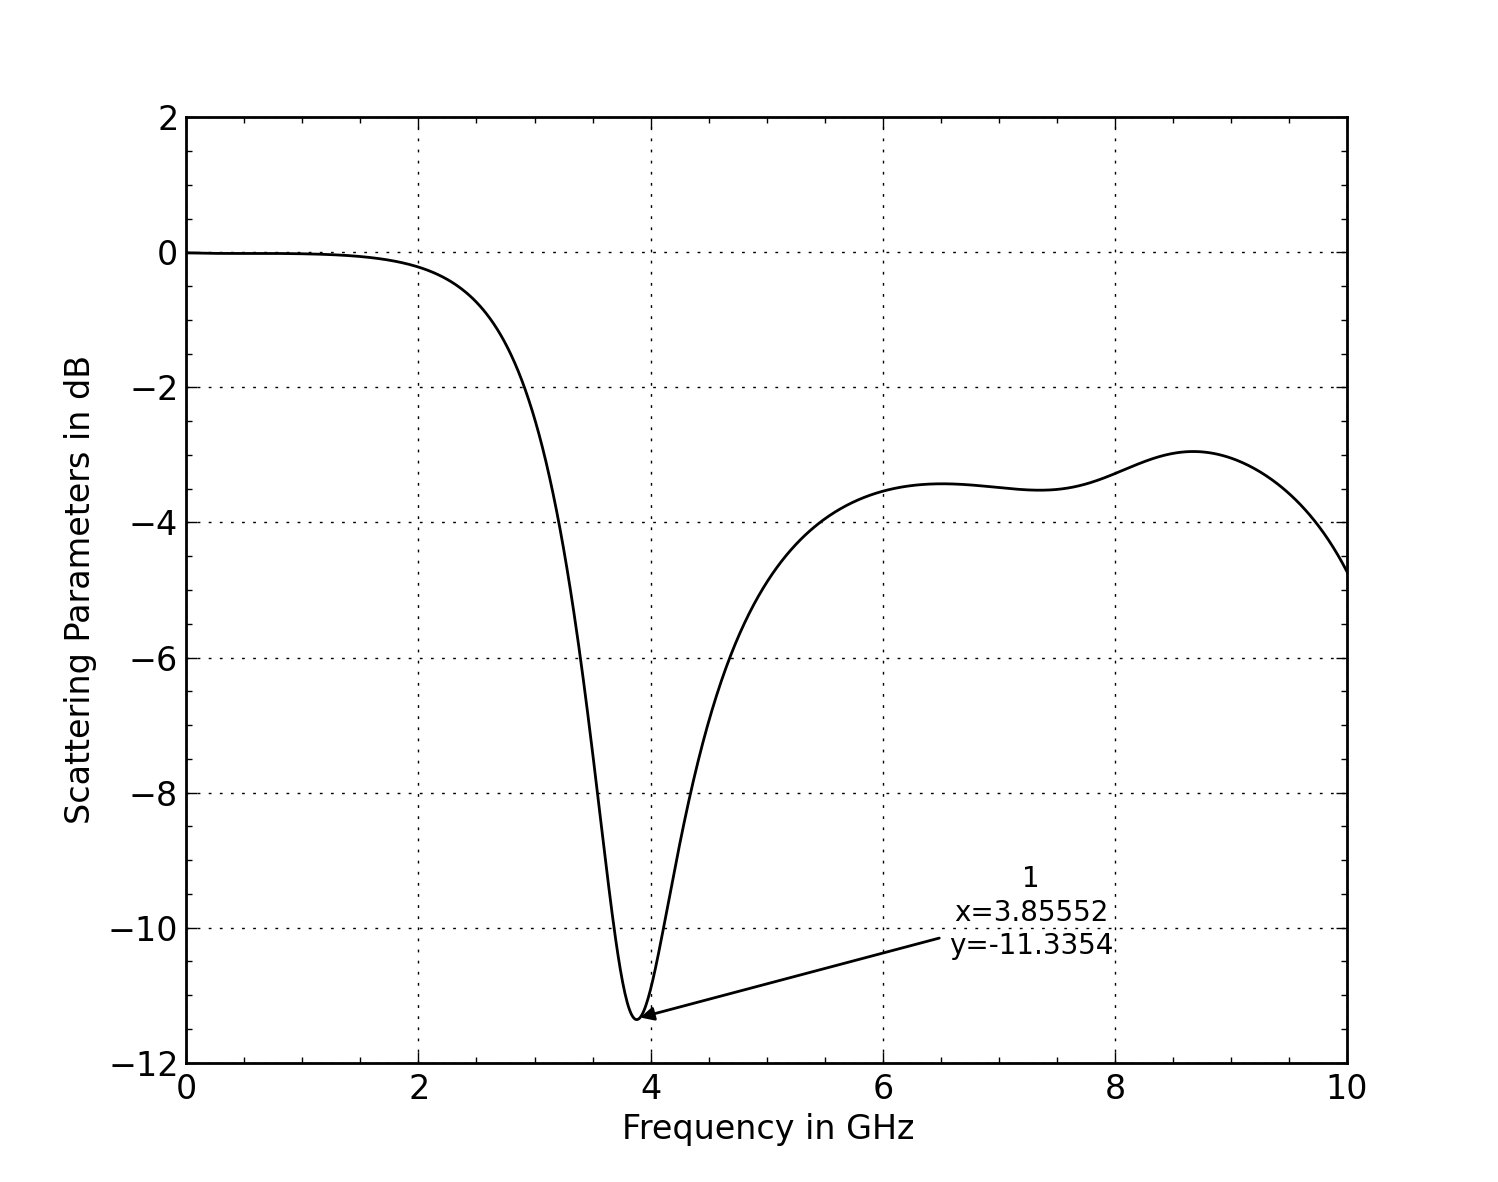
\includegraphics[width=0.75\textwidth]{../fig/plt/monopol_a_sim_s11.png}
	\caption{Reflexionskoeffizient ($S_{11}$ Parameter).}
\end{figure}

Die Simulation zeigt, dass die beste Abstrahlung leicht unter der
gewünschten Frequenz von \SI{4}{\giga\hertz} liegt. Dieses Ergebnis
kann nun in der Weise interpretiert werden, dass die erstellte
Antenne zu \emph{lang} ist. Durch die Kürzung der Stablänge $l_S$
kann dies korrigiert werden, denn damit wird die Wellenlänge
$\lambda$ reduziert und folglich die Frequenz erhöht.

\newpage
\subsubsection{Antennenimpedanz}

\begin{figure}[h!]
	\centering
	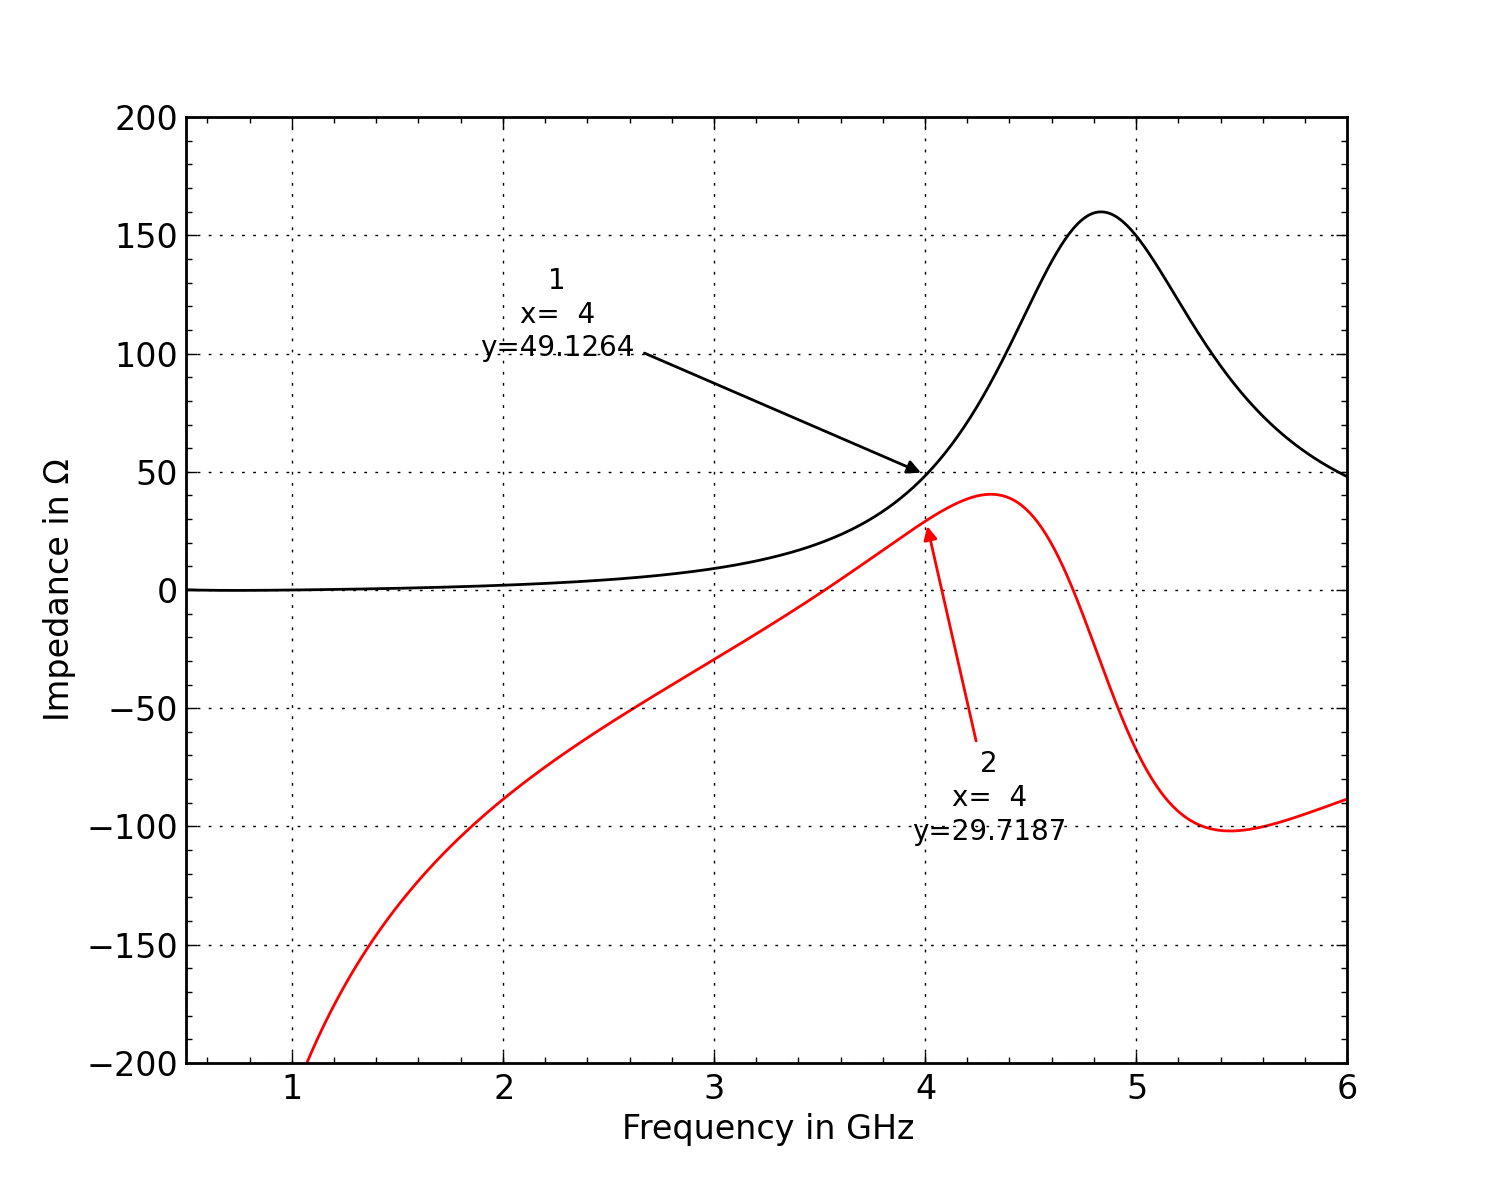
\includegraphics[width=0.75\textwidth]{../fig/plt/monopol_a_sim_impedance.png}
	\caption{Antennenimpedanz ($\mathrm{Re}\left\{Z\right\}$ schwarz,  $\mathrm{Im}\left\{Z\right\}$ rot).}
\end{figure}

Die Simulation zeigt, dass der Realanteil
$\mathrm{Re}\left\{Z\right\} \approx \SI{50}{\ohm}$ und somit dem
gewünschten Wert entspricht. Der Imaginäranteil ist mit
$\mathrm{Im}\left\{Z\right\} \approx \SI{30}{\ohm}$ deutlich über
dem geforderten Wert von \SI{0}{\ohm}, hat induktiven Charakter (da
$\mathrm{Im}\left\{Z\right\} > 0$) und bedeutet, dass eine suboptimale
Ausnutzung vorliegt (da ein Teil der Leistung nicht abstrahlungsfähig
ist durch die resultierende Reflexion). Weiter ist in der Abbildung ein
nahe liegener Resonanzpunkt zu erkennen bei ca. \SI{4.8}{\giga\hertz}.
Da dieser Resonanzpunkt nahe liegt und die Impedanz in dessen Umgebung
eine hohe Änderungsrate $\frac{\mathrm{d}Z}{\mathrm{d}f}$ besitzt,
bedeutet dies, dass die Impedanzverhältnisse nicht robust und die
Antenne \emph{empfindlich} ist auf eine Änderung der Frequenz $f$.
Die Simulation zeigt, dass eine Änderung der Frequenz um 
\SI{400}{\mega\hertz} den Realanteil der Impedanz bereits
verdoppelt auf \SI{100}{\ohm}.


\newpage
\subsubsection{2D Richtdiagramm}

\begin{figure}[h!]
	\centering
	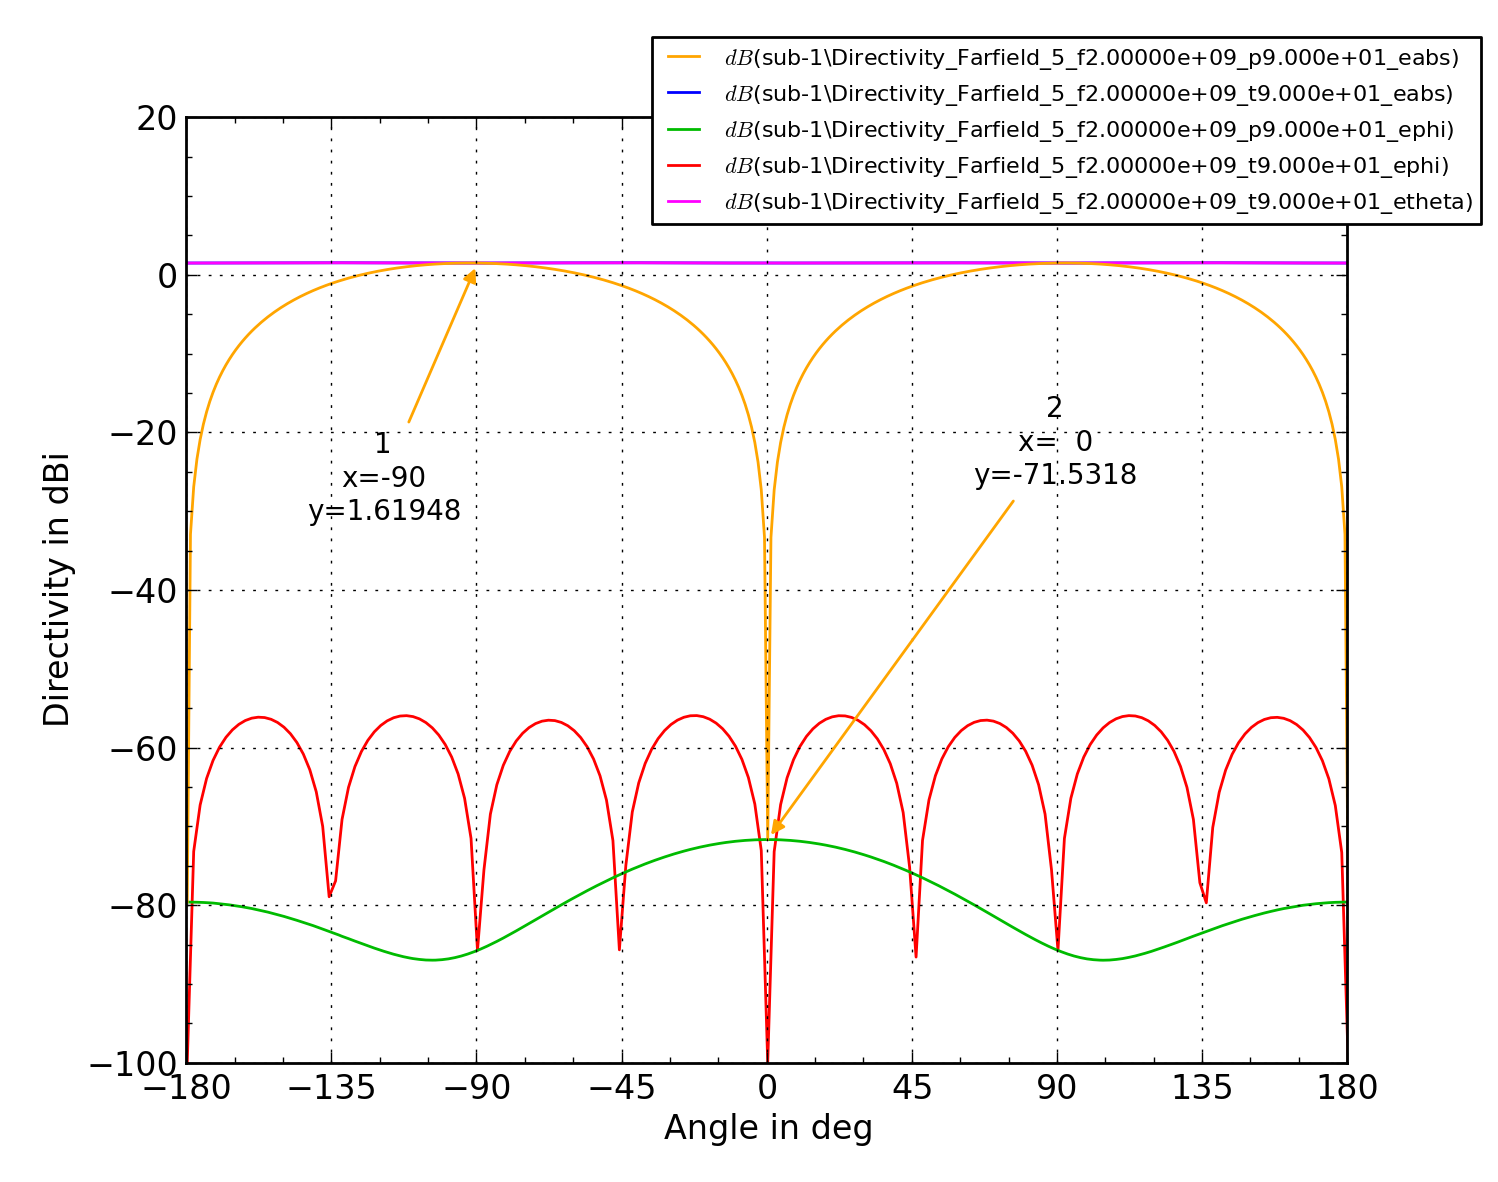
\includegraphics[width=0.75\textwidth]{../fig/plt/monopol_a_sim_2d_pattern.png}
	\caption{2D Richtdiagramm.}
\end{figure}

Die Simulation zeigt, dass die Antenne die erwatrete Abstrahlcharakteristik
eines idealen Monopols aufweist, welcher eine maximale Abstrahlung bei
$\pm \SI{90}{\degree}$ (senkrecht zum Stab) und die minimale Abstrahlung
bei \SI{0}{\degree} respektive \SI{180}{\degree} (entland des Stabs)
aufweist ($E_{\mathrm{abs}}$).

\newpage
\subsubsection{3D Richtdiagramm}

\begin{figure}[h!]
	\centering
	%\begin{subfigure}[b]{0.48\textwidth}
		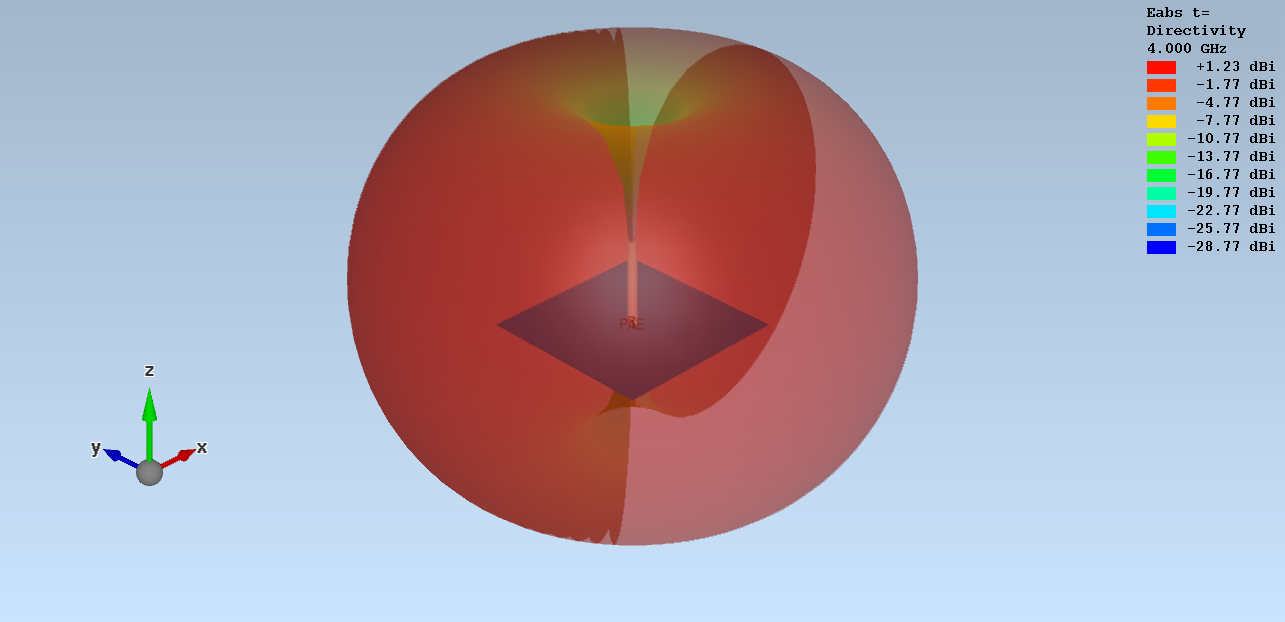
\includegraphics[width=1\textwidth]{../fig/plt/monopol_a_sim_3d_eabs.png}
	%	\caption{E-Feld Absolut}
	%\end{subfigure}
	%\begin{subfigure}[b]{0.48\textwidth}
	%	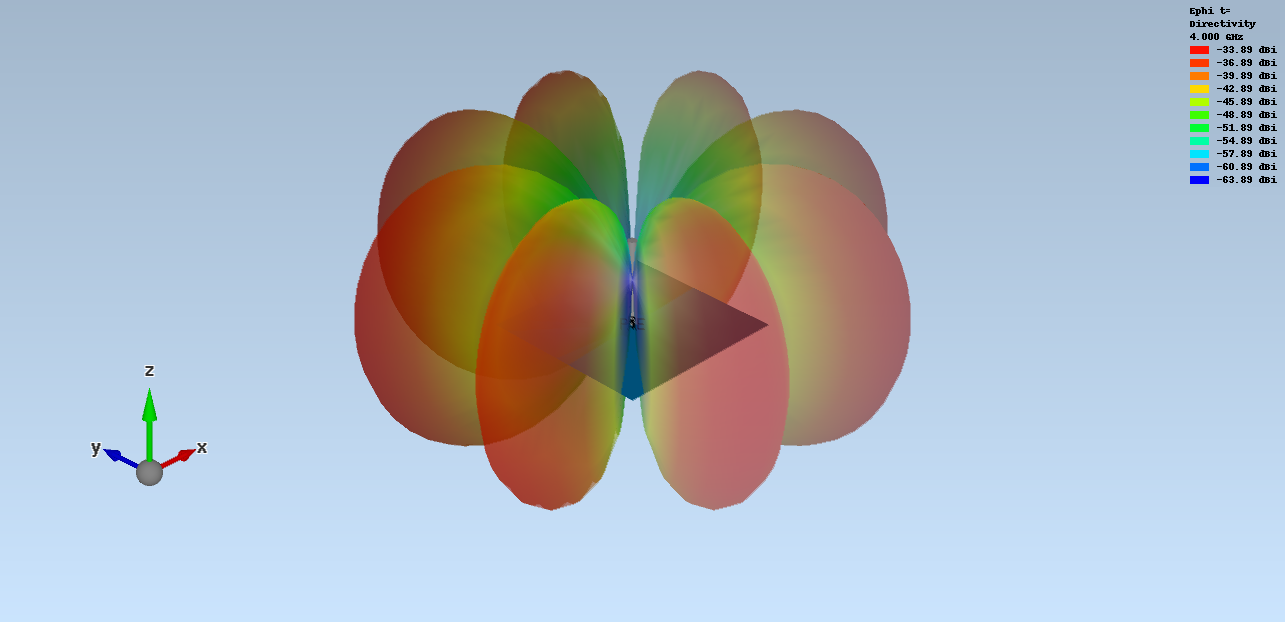
\includegraphics[width=1\textwidth]{../fig/plt/monopol_a_sim_3d_ephi.png}
	%	\caption{E-Feld $\varphi$}
	%\end{subfigure}
	\caption{3D Darstellung des Fernfeldes}
\end{figure}

Die Simulation zeigt wie bereits das 2D Richtdiagramm die Abstrahlung
der Antenne ($E_{\mathrm{abs}}$). Hier ist nochmals deutlich zu sehen,
dass die Antenne \emph{seitwärts} gut abstrahlt, \emph{auf-} und
\emph{abwärts} jedoch ein \emph{Funkloch} besteht.

\subsection{Messungen}

\subsubsection{Modell}

%\begin{figure}[h!]
%	\centering
%	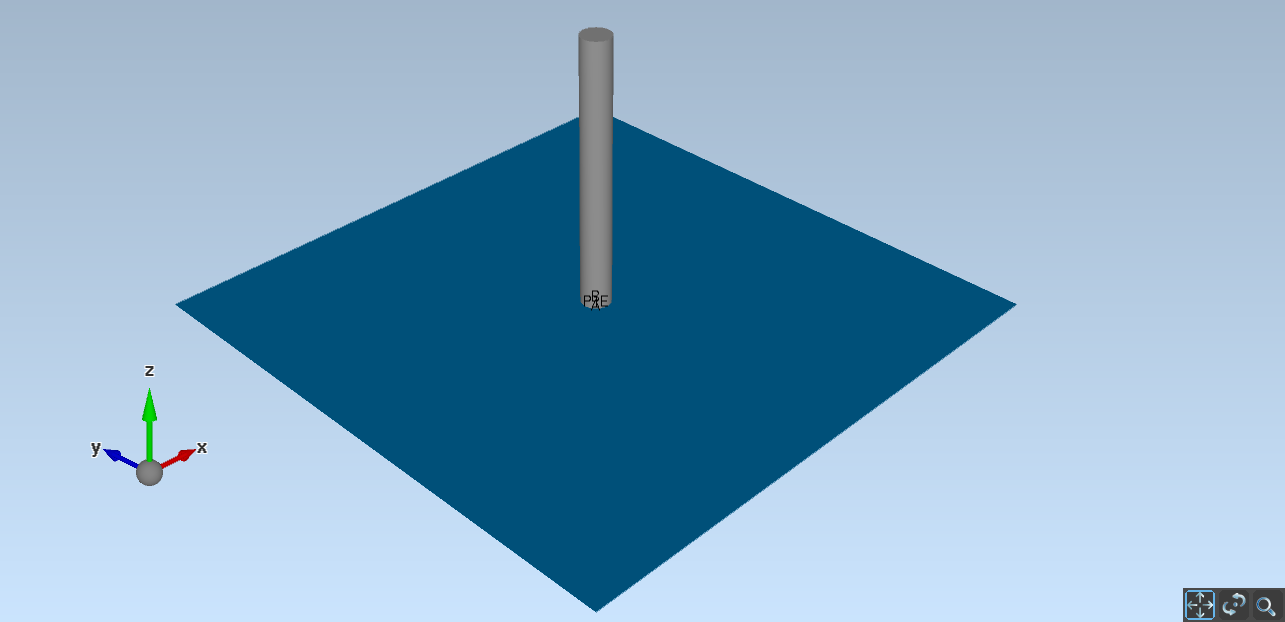
\includegraphics[width=0.5\textwidth]{../fig/plt/monopol_a_sim_3d_model.png}
%	\caption{}
%\end{figure}

\clearpage
\subsubsection{Messergebnisse}

\begin{figure}[h!]
	\begin{subfigure}[t]{0.45\textwidth}
		\centering
		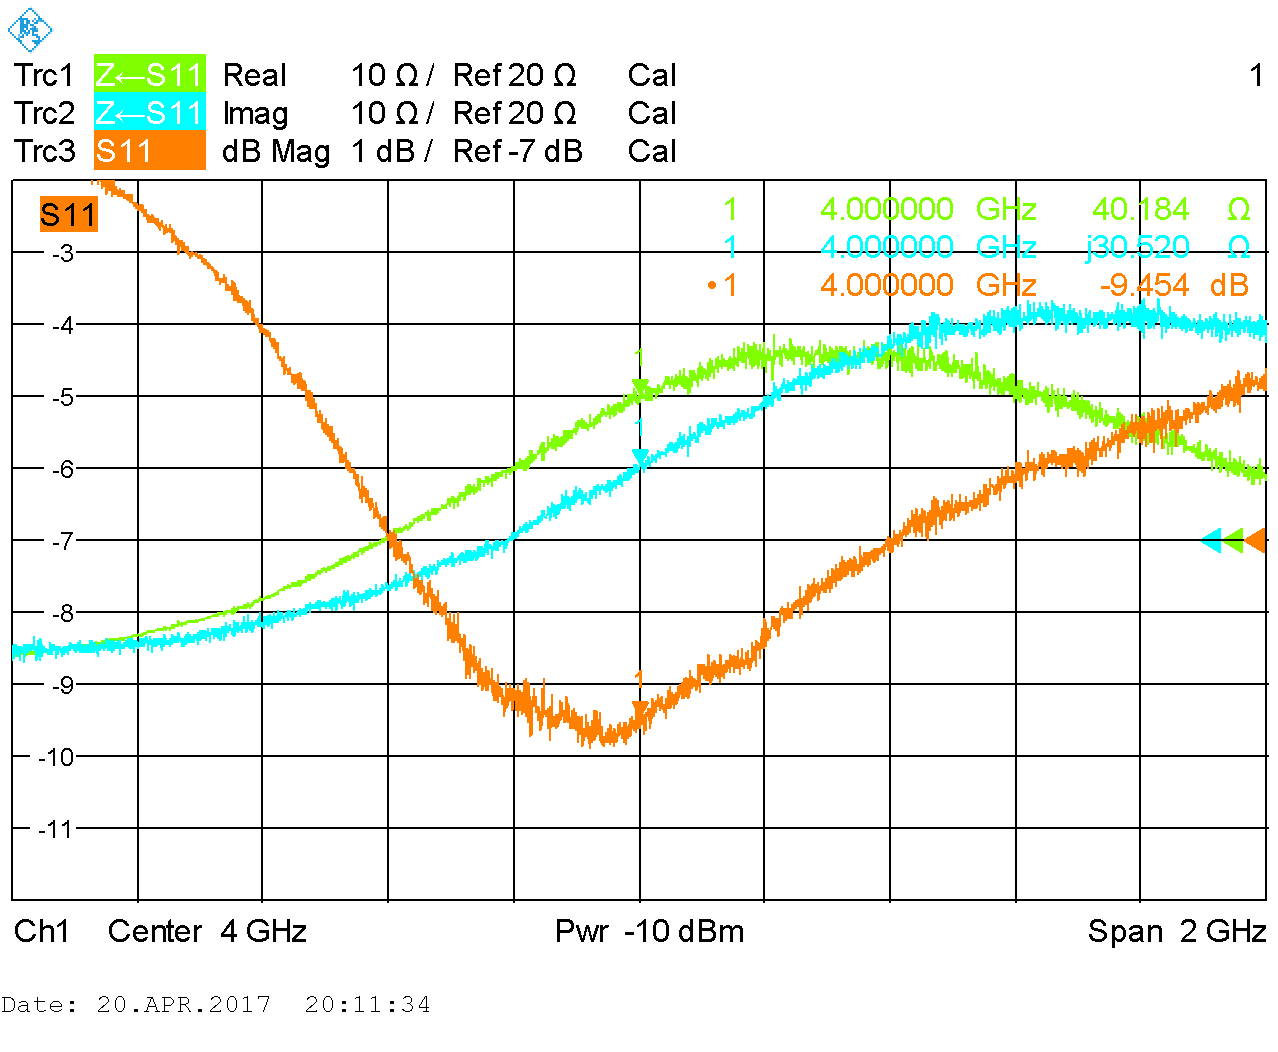
\includegraphics[width=1\textwidth]{../data/measurement/T2.png}
	\end{subfigure}
	\begin{subfigure}[t]{0.45\textwidth}
		\centering
		\begin{tikzpicture}
			\begin{axis}[
				title=\textbf{Reflexion $S_{11}$ (VNA2)},
				width=\linewidth,
				grid=major,
				grid style={dashed,gray!30},
				xlabel={Frequenz [\si{\giga\hertz}]},
				ylabel={$S_{11}$ [\si{\decibel}]},
				x label style={at={(axis description cs:0.5,-0.075)},anchor=north},
				legend style={at={(0.98,0.98)},anchor=north east},
				x tick label style={rotate=90,anchor=east},
				legend columns=1,
				]
				\addplot+[mark=none] table[x=f, y=s11, col sep=comma]{../data/measurement/vna_2_data.txt};
				%\addlegendentry{S11};
			\end{axis}
		\end{tikzpicture}
	\end{subfigure}
	\caption{Messung mit Vector-Nectorwork Analyser.}
\end{figure}

\subsubsection{Messaufbau}

\subsubsection{Messmittel}



%\subsection{Messgeräte}

\todo{Liste der verwndeten Messgeräte aufführen}

%\subsection{Messaufbau}

\todo{Messaufbau darlegen}



\clearpage
\section{Resultate}

\todo{Erreichte Messergebnisse, Antworten auf allfällige
	Fragestellungen, die mit Hilfe durchgeführter Messungen
	hergeleitet werden.}

\clearpage
\section{Diskussion}

\todo{Die wichtigsten Ergebnisse der Versuche werden in Worte qualitativ
	beschrieben und bewertet. Unstimmigkeiten zwischen den Ergebnissen
	einerseits und den allfällig berechneten / simulierten Grössen
	andererseits sollen diskutiert werden, und mögliche Ursachen als
	Hypothesen formuliert werden.}

\clearpage

\cite{ts}

% bibliography
\newpage
\cleardoublepage
\addcontentsline{toc}{section}{Literatur}
% \setlength\bibitemsep{1.5\itemsep}
%\nocite{*}
%\bibliographystyle{apacite}
\bibliographystyle{ieeetr}
%\bibliographystyle{pkg/deIEEEtran}
\bibliography{bib/bibliography}



% glossary
\newpage
\cleardoublepage

\clearpage
%\begin{multicols}{2}
%	\scriptsize
%	\glossarystyle{altlistgroup}
%	\glsaddall
%	\printglossary[title=Glossar]
	\printglossaries
%\end{multicols}

% list of figures
\clearpage
%\newpage
%\cleardoublepage
% \phantomsection
\addcontentsline{toc}{section}{Abbildungen}
\listoffigures

% lsit of tables
\clearpage
%\newpage
%\cleardoublepage
% \phantomsection
\addcontentsline{toc}{section}{Tabellen}
\listoftables

% appendix
\clearpage
\begin{appendices}
%\pagenumbering{roman}
\addtocontents{toc}{\protect\setcounter{tocdepth}{2}}

% appendix contents

%\clearpage

\end{appendices}

